\section{実験}
\subsection{共通設定}
評価にはCOCO 2017 Validationの5000枚を用いた．
画像の並びをseed 42で並べ替え，前半の2500枚（GTの物体18670件）を検証用，後半の2500枚（GTの物体17665件）をテスト用とした．
検証用の画像は類似度の下限値$ \theta $の選択にのみ用い，結果はテスト用の画像で報告する．
物体認識モデルは各画像に1回だけ適用し，YOLO11xは1画像あたり平均6.5件，DETRは平均11.2件のボックスをテスト用の画像で出力した．
GPUにはNVIDIA GeForce RTX 4070 Tiを用い，いずれのモデルも追加の学習は行わない．

\subsection{予備実験：COCOの80クラスによる基本の手法の評価}
本節では，3.1節の基本の手法を，学習時のクラスの範囲で評価する．
定量評価では，初期の語彙$ {\mathbb W} $をCOCOの80クラスのクラス名とし，下位語の集合は生成しない．
すなわち，Algorithm \ref{alg_granular}の最初の段階のみを行い，各ボックスにCOCOのクラスを1つ付けるか，類似度が$ \theta $未満のボックスを出力しない．
比較対象は，同じボックスに物体認識モデル自身が出力したクラスを付けたもの（以下，Close Vocabularyモデル）である．
同じ物体認識モデルのボックスを用いるため，提案手法とClose Vocabularyモデルの差は，クラスの推定の差のみとなる．

予測したボックスとGTのボックスは，IoUが0.5以上の組をハンガリアン法\cite{ref_Hungarian}で1対1に対応付けた．
同じボックスを用いるため，ボックスの位置や数は両者で等しく，比較にはクラスの推定のみを評価する指標が適する．
そこで，対応したボックスの数を$ N_{\mathrm{match}} $，そのうちクラスがGTと一致した数を$ N_{\mathrm{correct}} $とし，ラベルの一致率を

\begin{equation}
    A = \frac{N_{\mathrm{correct}}}{N_{\mathrm{match}}}
    \label{eq_metrics}
\end{equation}

\noindent
とした．
類似度による棄却は行わない（$ \theta = -1 $）．

テスト用の画像において，同じボックスに対するラベルの一致率$ A $は，Close VocabularyモデルのYOLO11xが0.970，DETRが0.955であるのに対し，YOLO11xのボックスではCLIPが0.572，SigLIPが0.582，DETRのボックスではCLIPが0.560，SigLIPが0.557であった．
すなわち，COCOの80クラスの範囲では，文章・画像埋め込みモデルによるゼロショット分類は，COCOで学習した物体認識モデルのクラスの推定に大きく劣った．
また，$ \theta $を大きくして類似度の低い予測を棄却すると，検証用の画像でラベルの一致率は0.91〜0.97まで向上したが，正しい予測も多く棄却された．
したがって，類似度の値のみでは正誤を区別しにくく，この問題は3.3節のスコアで扱う．

次に，定性評価では，初期の語彙$ {\mathbb W} $をWordNetの上位語とした．
WordNetの名詞の最上位のカテゴリ（noun.Tops）のうち，物体を表すperson，animal，plant，food，artifact，natural objectの6語を用いた．
テスト用の画像のうちGTの物体が2個以上6個以下の画像からseed 42で6枚を選び，棄却は行わない．
図\ref{fig_qualitative}に，YOLO11xのボックスに対する結果の一部を示す．

\begin{figure*}[t]
    \centering
    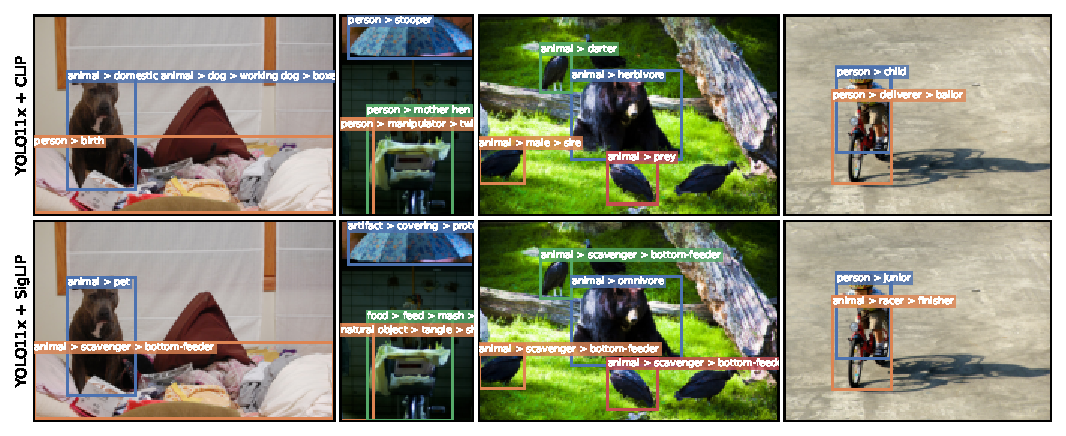
\includegraphics[width=0.8\linewidth]{figures/fig_qualitative.pdf}
    \caption{初期の語彙をWordNetの上位語6語とした定性評価の結果（上段：YOLO11x + CLIP，下段：YOLO11x + SigLIP，いずれも$ \theta = -1 $）．各ボックスに出力した単語の列を粗い語から順に示す．}
    \label{fig_qualitative}
\end{figure*}

図\ref{fig_qualitative}から，CLIPは犬をanimal → domestic animal → dog → working dog → boxerと，COCOのクラスであるdogを経由して犬種まで推定した．
SigLIPは傘をartifact → covering → protective covering → shade → parasolと推定した．
一方，同じ犬に対してSigLIPはanimal → petとし，熊にはanimal → omnivoreまたはherbivore，鳥にはanimal → scavenger → bottom-feederやanimal → preyが付けられた．
WordNetにおけるanimalの直接の下位語には，chordateのような分類学上の語に加えて，pet，herbivore，scavengerのように役割によって動物を分ける語が含まれ，これらの語にはさらに細かい下位語がほとんど無いため，細分化が浅い段階で止まった．
また，自転車にperson → deliverer → bailorやanimal → racer → finisherが付けられたように，最初の段階で物体と無関係な上位語を選ぶと，以降の単語も物体と無関係になった．

\subsection{COCO外の物体に対する評価の方法}
3.3節の提案手法を評価するため，COCOの画像に付与されたLVIS v1\cite{ref_LVIS}のアノテーションを用いた．
LVISは1203カテゴリのアノテーションを持ち，各カテゴリにWordNetのSynsetが付与されている．
LVISは，COCOで学習したYOLO11xをそのまま適用できるCOCOの画像に，COCOの80クラス以外の物体の正解とそのSynsetを与えるため，学習時に無い物体の命名を，上位語・下位語の関係を含めて自動で評価できる．
4.1節の検証用とテスト用の画像のうちLVISのアノテーションがある画像（検証用2387枚，テスト用2365枚）を用い，SynsetがCOCOのクラスのSynsetの上位語・下位語・自身のいずれでもなく，レンマもCOCOのクラス名と一致しない物体をCOCO外の物体（テスト用で13150件），それ以外をCOCOの物体（同11765件）とした．
出力したボックスとLVISのGTをIoU 0.5以上で1対1に対応付け，GTに出力が対応した割合を検出，出力した単語がGTのSynsetの上位語・自身・下位語のいずれかであった割合を命名，GTのSynset以下の単語まで細分化できた割合を細分化とした．
ただし，命名では深さ3未満の語とwholeを除いた．
また，出力した単語とGTのSynsetのそれぞれについて，自身と上位語のうち深さ3以上でwholeを除くSynsetの集合を求め，それらの重なりから階層的適合率$ hP $，階層的再現率$ hR $，およびその調和平均$ hF $を計算した\cite{ref_hF}．
GTと対応しない出力は全て誤りとし，このときの値を$ hP_{\mathrm{strict}} $，$ hF_{\mathrm{strict}} $とした．
ただし，LVISのアノテーションは全ての物体を網羅していないため，GTと対応しない出力には注釈の無い正しい物体も含まれる．
そこで上限の目安として，LVISの評価方法に倣い，画像に存在しないと確認されたカテゴリか，網羅的に注釈されたカテゴリの語またはその下位語を出力した場合のみ誤りとする$ hP_{\mathrm{fed}} $，$ hF_{\mathrm{fed}} $も求めた．
物体認識モデルにはYOLO11xを用い，3.3節の設定は検証用の画像で$ hF_{\mathrm{fed}} $が最大となるものを，$ \beta \in \{1, 2, 4, 8\} $，$ \tau \in \{0.05, 0.1, 0.2, \ldots, 0.9\} $，$ K \in \{10, 20, 50, 100\} $，$ o_{\min} \in \{0, 0.02, 0.05, 0.1, 0.2, 0.3\} $から，N1〜N4，A2の順に1段階ずつ選んだ．

OWLv2には，LVISの人手の注釈を学習に用いていないB/16の重み（自己学習のみ，以下ST）を主に用いた．
比較として，LVISの頻出カテゴリでファインチューニングした重み（以下FT）と，自己学習のみのL/14の重み（以下ST-L）も評価した．
FTは評価に用いるLVISのカテゴリの多くを学習時に見ているため，学習時に無い物体という本稿の目的に対しては参考値である．
なお，STもWeb上の画像と文章の大量の組による自己学習を行っているため，評価に用いる物体を一度も見ていないとは限らない．
本稿の「学習時に無い物体」は，LVISのカテゴリを正解のラベルとして学習していない物体を指す．

4.5節以降では，出力をスコアの順に並べた評価を行う．
スコアの高い順に出力をGTに対応付け（COCOのAPと同じ方法），スコアの閾値を下げながら出力を加えた場合の$ hR $と$ hP_{\mathrm{fed}} $，$ hP_{\mathrm{strict}} $から，適合率を単調にした曲線の面積をAP$ _{\mathrm{fed}} $，AP$ _{\mathrm{strict}} $とした．
階層的適合率・再現率は階層を持つ分類の評価に用いられる指標であり\cite{ref_hF}，粗い語の正しい出力に部分的な得点を与えるため，粒度を選ぶ手法の評価に適する．
本稿では，AP$ _{\mathrm{strict}} $を主な指標とし，AP$ _{\mathrm{fed}} $は上限の目安として示す．
一方，既存の物体認識の評価と比べるため，出力した単語がGTのSynset自身またはその下位語である出力のみを正解とするAP$ _{\mathrm{exact}} $も求めた．
AP$ _{\mathrm{exact}} $は，GTと対応しない出力を全て誤りとし，カテゴリを区別せずに全ての出力を1つの順位に並べたIoU 0.5のAPであり，LVISのカテゴリまで細分化した出力のみを正解とするため，通常のオープンボキャブラリの物体認識の評価に近い．
また，画像を単位として1000回の復元抽出を行うブートストラップ\cite{ref_Bootstrap}により，テスト用の画像における手法の間の差の95\%信頼区間を求めた．

\subsection{分類の能力と設定の影響}

\begin{table}[t]
    \vspace{3mm}
    \centering
    \caption{加えた領域のうちCOCO外の物体と重なるものについて，OWLv2の1位の単語が正しかった割合（テスト用）．括弧内は正しい上位語・下位語を含む割合である．LVISの語彙は正解の語を必ず含む．}
    \label{tab_diag}
    \footnotesize
    \begin{tabular}{lccc}
        \toprule
        OWLv2 & 領域数 & LVIS（1202語） & キャプション（7806語） \\
        \midrule
        ST & 1869 & 0.411 (0.468) & 0.180 (0.241) \\
        ST-L & 1450 & 0.438 (0.496) & 0.170 (0.218) \\
        FT & 3812 & 0.705 (0.762) & 0.477 (0.560) \\
        \bottomrule
    \end{tabular}
\end{table}

表\ref{tab_diag}に，加えた領域（$ K = 10 $）のうちCOCO外の物体と重なるものに対する，OWLv2の分類の正解率を示す．
FTはLVISの語彙で70.5\%であったのに対し，STは41.1\%，ST-Lは43.8\%であり，以前の版で観測した高い分類能力の多くはLVISによるファインチューニングに由来していた．
また，正解を含む1202語から7806語に語彙を広げると，正解率はSTで18.0\%に下がった．
したがって，学習時に無い物体を扱う条件では，語彙全体からの1語の選択は信頼できず，確信度に応じて粗い語で止める必要がある．

\begin{table}[t]
    \vspace{3mm}
    \centering
    \caption{STを用いた場合のテスト用の画像における評価．各行は1つ上の行の設定に変更を加えたものである．$ hF_{\mathrm{fed}} $は設定の選択に用いた指標である．}
    \label{tab_open}
    \footnotesize
    \setlength{\tabcolsep}{2pt}
    \begin{tabular}{lcccc}
        \toprule
        & \multicolumn{3}{c}{COCO外の物体} & \\
        \cmidrule(lr){2-4}
        構成 & 検出 & 命名 & 細分化 & $ hF_{\mathrm{fed}} $ \\
        \midrule
        flat & 0.212 & 0.034 & {\bf 0.033} & 0.377 \\
        deepest & 0.212 & 0.057 & 0.022 & 0.380 \\
        backoff & 0.212 & {\bf 0.063} & 0.013 & 0.386 \\
        greedy (N3) & 0.212 & 0.053 & 0.014 & 0.391 \\
        + N4 & 0.212 & 0.055 & 0.019 & 0.395 \\
        \midrule
        + $ K{=}20 $ & 0.302 & 0.094 & 0.034 & 0.423 \\
        + $ K{=}50 $ & 0.454 & 0.164 & 0.056 & 0.466 \\
        + $ K{=}100 $$ ^\dagger $ & {\bf 0.560} & {\bf 0.211} & {\bf 0.073} & {\bf 0.494} \\
        \bottomrule
    \end{tabular}
\end{table}

表\ref{tab_open}に，STを用いた場合の各段階の結果を示す（$ K = 10 $から開始し，$ ^\dagger $は$ o_{\min} = 0.02 $）．
確率が最大の単語をそのまま出力するflatは細分化が最も高いが命名は3.4\%であり，誤った細かい語が多かった．
上位語への集約（N2）と組み合わせると命名は5.3〜6.3\%に上がり，検証用の画像ではgreedy（$ \beta = 2 $，$ \tau = 0.1 $）が選ばれた．
語義を区別する文章と人の役割の除外（N4）により，細分化は1.4\%から1.9\%に向上した．
YOLO11xのボックスをクラスの下位語へ細分化する設定も評価したが，検証用の画像では細分化しない設定が選ばれた．
最も効果が大きかったのは加える領域の数$ K $であり，$ K = 100 $でCOCO外の物体の検出は21.2\%から56.0\%に，命名は5.5\%から21.1\%に，細分化は1.9\%から7.3\%に向上した．
一方で，加えた領域の多くは物体でない領域であった（4.7節）．

$ K $と$ o_{\min} $を$ hF_{\mathrm{strict}} $で選ぶと$ o_{\min} = 0.3 $となり，加える領域は1画像あたり2.0件に減り，COCO外の物体の命名は1.8\%にとどまった．
同じ設定（$ K = 100 $）で，ST-Lでは細分化が13.3\%とSTより高く，命名はSTと同程度の20.3\%であった．
FTでは命名35.5\%，細分化28.1\%となり，STとの差はLVISによるファインチューニングの効果を含む．
このように，$ K $と$ o_{\min} $のみでは命名を保ちながら誤った出力を減らすことは難しく，4.6節ではスコアによって出力を選ぶ．

\subsection{命名の方法の比較}
上位語への集約と確信度に応じた停止の効果を，階層を用いずに確率が最大の1語を出力する方法（flat）と比較した．
さらに，評価の語彙を事前に知る場合の参考として，OWLv2にLVISの1203カテゴリ名を語彙として与え，同じ2つの規則で命名した場合も評価した．
これは，評価するクラスの集合を与えるという，オープンボキャブラリの物体認識モデルの通常の使い方に相当する．
いずれもYOLO11xのボックスの出力は同じであり，加えた領域（$ K = 100 $）の命名のみが異なる．
各方法には，3.3節の(\ref{eq_score})のスコアを方法ごとに検証用の画像で重みを求めて付け，スコアの順の曲線で比較した．

\begin{table}[t]
    \vspace{3mm}
    \centering
    \caption{命名の方法ごとのテスト用の画像における評価．スコアは(\ref{eq_score})である．LVISの語彙は評価のカテゴリ名を事前に与える場合（参考）である．AP$ _{\mathrm{fed}} $は上限の目安である．}
    \label{tab_baseline}
    \footnotesize
    \setlength{\tabcolsep}{3pt}
    \begin{tabular}{lllccc}
        \toprule
        OWLv2 & 語彙 & 規則 & AP$ _{\mathrm{strict}} $ & AP$ _{\mathrm{exact}} $ & AP$ _{\mathrm{fed}} $ \\
        \midrule
        ST & キャプション & flat & 0.193 & {\bf 0.104} & 0.306 \\
         & キャプション & greedy & {\bf 0.197} & 0.096 & {\bf 0.333} \\
         & LVIS & flat & 0.209 & 0.116 & 0.351 \\
         & LVIS & greedy & 0.208 & 0.111 & 0.354 \\
        \midrule
        ST-L & キャプション & flat & 0.188 & {\bf 0.104} & 0.310 \\
         & キャプション & greedy & {\bf 0.191} & 0.102 & {\bf 0.331} \\
         & LVIS & flat & 0.203 & 0.119 & 0.362 \\
         & LVIS & greedy & 0.205 & 0.118 & 0.367 \\
        \midrule
        FT & キャプション & flat & 0.264 & 0.160 & 0.430 \\
         & キャプション & greedy & {\bf 0.277} & {\bf 0.161} & {\bf 0.456} \\
         & LVIS & flat & 0.316 & 0.220 & 0.511 \\
         & LVIS & greedy & 0.313 & 0.215 & 0.508 \\
        \bottomrule
    \end{tabular}
\end{table}

表\ref{tab_baseline}に結果を示す．
キャプションの語彙では，greedyはflatに比べ，全ての重みでAP$ _{\mathrm{strict}} $が0.003〜0.013高かった．
ブートストラップによる差の95\%信頼区間は，STで0.001〜0.009，FTで0.008〜0.019であり，いずれも0を含まなかったが，差は小さい．
一方，LVISのカテゴリまで正しい出力のみを数えるAP$ _{\mathrm{exact}} $は，STでflatの方が0.008（95\%信頼区間0.007〜0.010）高く，FTでは差が無かった（$-0.003$〜0.005）．
これは，greedyが確信度の低い領域で粗い語に止まり，細かい語での正解を一部失うためである．

この違いを領域ごとに確かめるため，テスト用の画像で検出のスコアの順にCOCO外の物体と対応した加えた領域（STで6385件）について，同じ領域に対する2つの方法の命名の正誤を比べた．
命名が正しかった割合は，flatの25.9\%に対しgreedyで43.0\%であった．
greedyのみが正しかった領域は1551件，flatのみが正しかった領域は457件であり，前者には，jerseyに対するflatのjerseyとgreedyのshirt，skirtに対するshort pantsとgarment，ringに対するbandとjewelryのように，flatが誤った細かい語を選び，greedyが正しい上位語に止まった例が多かった．
後者には，handleに対するknobとfastenerのように，greedyが最初の段階で誤った枝に進んだ例が多かった．
ST-Lでは42.2\%と29.7\%，FTでは56.2\%と48.9\%であり，分類の能力が高い重みほど差は小さかった．
すなわち，上位語への集約は領域ごとの命名の正しさを大きく改善するが，その多くは粗い語による正解であり，出力全体のAPへの寄与は小さい．

また，評価の語彙を事前に与えると，AP$ _{\mathrm{strict}} $はSTで0.193〜0.197から0.208〜0.209に，FTで0.264〜0.277から0.313〜0.316に向上した．
語彙が1203語に限られ正解の語を必ず含む場合には，greedyとflatの差は小さく，FTではflatが有意に高かった（AP$ _{\mathrm{strict}} $で0.003，95\%信頼区間0.001〜0.004）．
したがって，上位語への集約が有効なのは，評価の語彙を事前に知らず，大きな語彙から命名する場合である．

\subsection{アノテーションのスコアの評価}
3.3節のスコアの効果を評価するため，4.4節で選んだ設定（$ K = 100 $，$ o_{\min} = 0 $）の全ての出力にスコアを付け，4.3節のAP$ _{\mathrm{strict}} $とAP$ _{\mathrm{fed}} $を求めた．
また，スコアを確率とみなし，正誤が判定できる出力（GTと対応した出力と，$ hF_{\mathrm{fed}} $で誤りとした出力）について，10個のビンで期待校正誤差（Expected Calibration Error，ECE）\cite{ref_Calibration}を求めた．
比較として，学習を伴わない検出のスコア$ c({\mathbf b}) $，命名の確率$ q(n \mid {\mathbf b}) $，両者の積，および加えた領域のみ両者の積とする場合を評価した．
(\ref{eq_score})の重みは検証用の画像の18488件の出力（正の割合45.7\%）で求めた．

\begin{table}[t]
    \vspace{3mm}
    \centering
    \caption{スコアの種類ごとのテスト用の画像における評価．$ ^\dagger $は加えた領域のみ積とし，YOLO11xのボックスは$ c $とした場合である．AP$ _{\mathrm{fed}} $は上限の目安である．}
    \label{tab_score}
    \footnotesize
    \setlength{\tabcolsep}{4pt}
    \begin{tabular}{llccc}
        \toprule
        OWLv2 & スコア & AP$ _{\mathrm{strict}} $ & ECE & AP$ _{\mathrm{fed}} $ \\
        \midrule
        ST & $ c $ & 0.171 & 0.145 & 0.323 \\
        ST & $ q $ & 0.042 & 0.339 & 0.272 \\
        ST & $ c \cdot q $ & 0.116 & 0.436 & 0.301 \\
        ST & $ c \cdot q^\dagger $ & 0.171 & 0.231 & 0.324 \\
        ST & $ s $ & {\bf 0.197} & {\bf 0.028} & {\bf 0.333} \\
        \midrule
        ST-L & $ c $ & 0.162 & 0.146 & 0.320 \\
        ST-L & $ s $ & 0.191 & 0.025 & 0.331 \\
        FT & $ c $ & 0.243 & 0.168 & 0.438 \\
        FT & $ s $ & 0.277 & 0.013 & 0.456 \\
        \bottomrule
    \end{tabular}
\end{table}

\begin{figure*}[t]
    \centering
    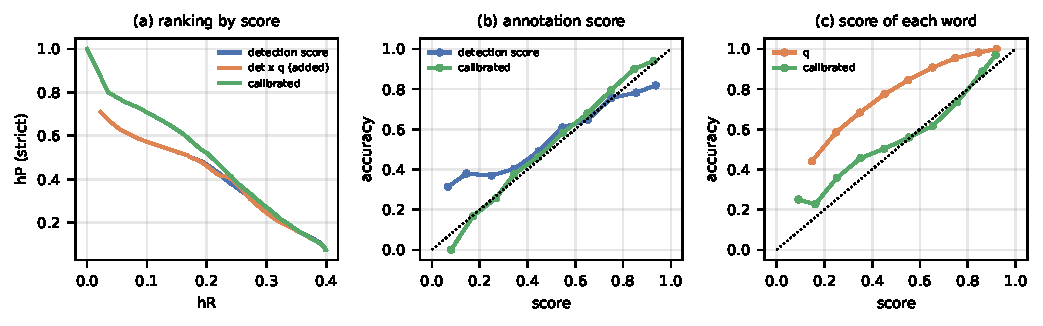
\includegraphics[width=0.8\textwidth]{figures/fig_score.pdf}
    \caption{STを用いた場合のテスト用の画像におけるスコアの評価．(a)スコアの順に出力を加えた場合の$ hR $と$ hP_{\mathrm{strict}} $，(b)アノテーションのスコアの値（横軸）と正解率（縦軸）の関係，(c)GTと対応した加えた領域の経路上の各単語の集約した確率$ q $と(\ref{eq_word_score})のスコアの値と正解率の関係．点線は完全に校正された場合である．}
    \label{fig_score}
\end{figure*}

表\ref{tab_score}と図\ref{fig_score}に結果を示す．
命名の確率$ q $のみでは，物体でない領域にも高い値が付くためAP$ _{\mathrm{strict}} $は0.042と低く，検出のスコアとの積でもYOLO11xのボックスの$ q $が低いため検出のスコアのみより低下した．
加えた領域のみ積とすると，学習を伴わずに検出のスコアと同程度以上となった．
(\ref{eq_score})のスコア$ s $は，全ての重みでAP$ _{\mathrm{strict}} $とAP$ _{\mathrm{fed}} $が最も高く，STではAP$ _{\mathrm{strict}} $が0.171から0.197に向上した．
また，ECEは0.145から0.028に低下し，図\ref{fig_score}(b)のようにスコアの値が正解率とほぼ一致した．
経路上の各単語では，集約した確率$ q $は正解率より低く（ECE 0.275），(\ref{eq_word_score})のスコアによりECEは0.041に低下した（ST-Lで0.172から0.062，FTで0.244から0.041）．
この改善は偶然によるものではなく，ブートストラップによるSTのAP$ _{\mathrm{strict}} $の差は0.026（95\%信頼区間0.021〜0.031），FTでは0.034（0.028〜0.041）であった．

\begin{figure*}[t]
    \centering
    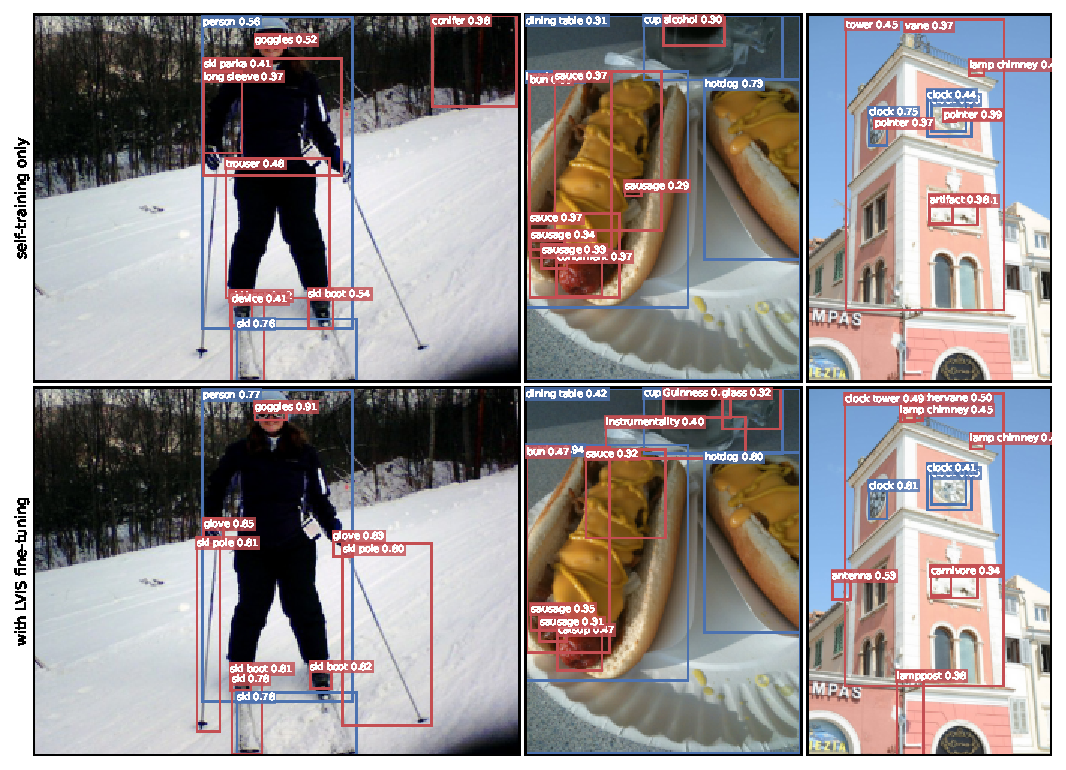
\includegraphics[width=0.62\textwidth]{figures/fig_qualitative_open.pdf}
    \caption{テスト用の画像における出力の例（上段：ST，下段：FT）．青はYOLO11xのボックスとクラス，赤は加えた領域のうち(\ref{eq_score})のスコアが高い上位8件と，3.3節の方法で選んだ単語，数値はそのスコアである．}
    \label{fig_qualitative_open}
\end{figure*}

図\ref{fig_qualitative_open}に出力の例を示す．
STでも，スキーの画像のgoggles（0.52），ski boot（0.54），trouser（0.48），ski parka（0.41），ホットドッグの画像のsausage，sauce，時計塔の画像のtower（0.45）のように，COCO外の物体に正しい単語とスコアが付けられた．
例えばski parkaの領域の経路上の各単語のスコアは，artifact 0.89，clothing 0.89，jacket 0.82，parka 0.62，ski parka 0.43であり，粗い語ほど高い．
一方，STではalcohol（0.30）のような誤りも残り，FTではgoggles（0.91），glove（0.85），ski pole（0.81）のように正しい細かい語に高いスコアが付けられた．

\subsection{誤りの分解}
提案手法の精度を制限する要因を調べるため，テスト用の画像における加えた領域の出力を，スコアの順にGTへ対応付けた結果から6種類に分けた．
GTと対応し命名が正しい出力を正しい命名，GTと対応したが命名が誤りの出力を誤った命名，IoUが0.5以上のGTが既に他の出力に対応していた出力を重複とした．
GTと対応しない残りの出力は，領域の面積の80\%以上がいずれかのGTのボックスに含まれる場合を物体の一部，GTとの最大のIoUが0.1以上0.5未満の場合を位置ずれ，それ以外を背景とした．
ただし，LVISのアノテーションは網羅的でないため，物体の一部と背景には注釈の無い物体も含まれる．

\begin{table}[t]
    \vspace{3mm}
    \centering
    \caption{加えた領域の出力の種類の割合（\%，テスト用）．「全て」は$ K = 100 $の全ての出力，「閾値」は検証用の画像で$ hF_{\mathrm{strict}} $が最大となる(\ref{eq_score})の閾値以上の出力である．}
    \label{tab_errors}
    \footnotesize
    \setlength{\tabcolsep}{1.5pt}
    \begin{tabular}{lccccccc}
        \toprule
        構成 & 出力数 & 正しい & 誤り & 重複 & 一部 & 位置 & 背景 \\
        \midrule
        ST greedy 全て & 220899 & 1.8 & 2.3 & 0.5 & 35.0 & 9.8 & 50.8 \\
        ST greedy 閾値 & 4657 & 16.6 & 5.8 & 0.9 & 31.1 & 13.0 & 32.6 \\
        ST flat 閾値 & 3763 & 17.3 & 11.0 & 0.7 & 28.2 & 14.8 & 27.9 \\
        FT greedy 閾値 & 14489 & 26.6 & 10.0 & 0.4 & 23.2 & 8.4 & 31.5 \\
        \bottomrule
    \end{tabular}
\end{table}

表\ref{tab_errors}に結果を示す．
STで$ K = 100 $の全ての出力のうち，GTと対応した出力は4.1\%にすぎず，物体の一部が35.0\%，背景が50.8\%を占めた．
閾値以上の出力に限っても，物体の一部，位置ずれ，背景の合計は76.7\%であり，誤った命名は5.8\%であった．
flatでは誤った命名が11.0\%とgreedyの約2倍であり，greedyは命名の誤りを粗い語に止まることで減らしていた．
すなわち，提案手法の誤りの多くは，命名ではなく，物体の全体でない領域を加えることに起因する．

この要因の大きさを見積もるため，GTを用いて，いずれかのGTとIoUが0.5以上で重なる加えた領域のみを残した場合を評価した．
これはGTを用いるため手法ではなく，領域の追加が完全な場合の上限である．
STで(\ref{eq_score})のスコアを用いると，AP$ _{\mathrm{strict}} $はgreedyで0.197から0.265に，flatで0.193から0.237に向上した．
物体でない領域が除かれると，greedyとflatの差はAP$ _{\mathrm{strict}} $で0.004から0.028に広がった．
ST-Lでは0.264と0.239，FTでは0.401と0.365であり，FTではAP$ _{\mathrm{exact}} $もgreedyが0.228とflatの0.222を上回った．
したがって，物体でない領域を区別する方法が得られれば，上位語への集約による命名の改善が出力全体の精度により大きく反映される．

\begingroup
\color{red}
\begin{table}[t]
    \vspace{3mm}
    \centering
    \caption{\add{全体らしさの特徴を(\ref{eq_score})に加えた場合のAP$ _{\mathrm{strict}} $（テスト用，greedy）．括弧内は加えない場合との差の95\%信頼区間である．}}
    \label{tab_whole}
    \color{red}
    \footnotesize
    \setlength{\tabcolsep}{2pt}
    \begin{tabular}{lcccc}
        \toprule
        特徴 & \multicolumn{2}{c}{ST} & \multicolumn{2}{c}{FT} \\
        \midrule
        加えない & 0.197 & --- & 0.277 & --- \\
        ＋幾何 & 0.200 & [$+$0.002, $+$0.004] & 0.280 & [$+$0.001, $+$0.004] \\
        ＋WordNet & 0.196 & [$-$0.003, 0.000] & 0.274 & [$-$0.005, $-$0.001] \\
        ＋両方 & 0.199 & [0.000, $+$0.003] & 0.276 & [$-$0.003, 0.000] \\
        規則で棄却 & 0.197 & [0.000, $+$0.001] & 0.277 & [$-$0.002, $+$0.001] \\
        \bottomrule
    \end{tabular}
\end{table}

そこで，GTを用いずに物体の全体でない領域を区別することを試みた．
加えた領域ごとに，面積が1.5倍以上のYOLO11xのボックスおよび全てのボックスに含まれる割合の最大値，内側に含む加えた領域の数，画像内で最大のボックスに対する面積の比の4個を幾何の特徴とした．
また，面積の80\%以上を含む大きなボックスの経路上の語の部分（WordNetのpart meronymを推移的にたどったもの）に出力した語が当たるか，および出力した語が何かの部分を表す語かの2個をWordNetの特徴とした．
例えば，carのボックスに含まれるwheelの領域は前者が真となる．
これらを(\ref{eq_score})の特徴に加えて検証用の画像で重みを求め直した場合と，前者が真の領域を棄却する規則のみの場合の結果を表\ref{tab_whole}に示す．
幾何の特徴によりAP$ _{\mathrm{strict}} $はSTとFTで約0.002向上したが，ST-Lでは0.191から0.189に低下し，WordNetの特徴はいずれの場合も精度を向上させなかった．
part meronymが真となった領域のうち正しい出力は1〜2\%にすぎなかったが，物体の一部の出力のうち該当するものは9〜11\%であり，規則による棄却でも閾値以上の出力に占める物体の一部の割合は31.1\%から28.5\%に減るのみであった．
また，正しい出力の領域もYOLO11xのボックスに含まれる割合が平均0.63と高く（物体の一部は0.86），人の衣服のように大きな物体に含まれる物体と，物体の一部とを位置関係と語の関係のみでは区別できなかった．
\endgroup
